% ── Figure 1: System Architecture ─────────────
\begin{figure*}[t]
\centering
\begin{tikzpicture}[
  every node/.style={font=\small},
  box/.style={
    rectangle, rounded corners=5pt,
    draw=black!60, thick,
    minimum width=2.8cm,
    minimum height=1.0cm,
    align=center, fill=white},
  modelbox/.style={
    rectangle, rounded corners=5pt,
    draw=orange!70, thick,
    minimum width=3.2cm,
    minimum height=0.9cm,
    align=center, fill=orange!8},
  chainbox/.style={
    rectangle, rounded corners=5pt,
    draw=gray!60, thick,
    minimum width=2.8cm,
    minimum height=1.0cm,
    align=center, fill=gray!8},
  outbox/.style={
    rectangle, rounded corners=5pt,
    draw=green!50!black!60, thick,
    minimum width=2.8cm,
    minimum height=1.0cm,
    align=center, fill=green!6},
  arrow/.style={-Stealth, thick, draw=black!70},
  dasharrow/.style={-Stealth, thick,
    draw=black!40, dashed},
  node distance=1.2cm and 1.6cm
]

% ── Row 1: User-facing components ─────────────
\node[box, fill=blue!8] (fe) at (0,0)
  {\textbf{React/Electron}\\Frontend};

\node[box, fill=blue!8] (be) at (4.2,0)
  {\textbf{FastAPI Backend}\\localhost:8000};

\node[chainbox] (bc) at (4.2,-2.2)
  {\textbf{Ganache Node}\\port 7545};

\node[outbox] (out) at (0,-2.2)
  {\textbf{Redacted Output}\\+ \texttt{.audit.json}};

% ── Row 2: GPU models ─────────────────────────
\node[modelbox] (vlm) at (8.8, 0.9)
  {\textbf{Qwen2-VL-2B}\\VLM (1.40\,GB)};

\node[modelbox] (txt) at (8.8,-0.1)
  {\textbf{Qwen2.5-3B}\\Text (1.91\,GB)};

\node[modelbox] (ocr) at (8.8,-1.1)
  {\textbf{EasyOCR}\\GPU-accelerated};

\node[modelbox] (yolo) at (8.8,-2.1)
  {\textbf{YOLOv8n}\\Face detection};

% ── GPU bounding box ──────────────────────────
\node[draw=orange!70, very thick, dashed,
  rounded corners=8pt,
  fill=orange!3,
  fit=(vlm)(txt)(ocr)(yolo),
  inner sep=10pt,
  label={[font=\small\bfseries,
    text=orange!80!black]above:
    NVIDIA RTX 5060 Laptop GPU \ \
    8\,GB VRAM \ \ Peak: 3.31\,GB}
] (gpu) {};

% ── Outer system boundary ─────────────────────
\node[draw=black!50, very thick,
  rounded corners=10pt,
  fit=(fe)(be)(bc)(out)(gpu),
  inner sep=18pt,
  label={[font=\small\bfseries,
    text=black!60]above left:
    \textbf{Local Device} (no data leaves)}
] (system) {};

% ── Arrows ────────────────────────────────────
% Frontend <-> Backend
\draw[arrow] (fe.east) -- (be.west)
  node[midway, above, font=\footnotesize]
  {upload};
\draw[arrow] (be.west) -- (fe.east)
  node[midway, below, font=\footnotesize]
  {result};

% Backend -> Ganache
\draw[arrow] (be.south) -- (bc.north)
  node[midway, right, font=\footnotesize]
  {anchor};

% Backend -> Output
\draw[arrow] (be.south west) -- (out.north east)
  node[midway, below right, font=\footnotesize]
  {write};

% Frontend -> Output (display)
\draw[dasharrow] (fe.south) -- (out.north)
  node[midway, left, font=\footnotesize]
  {display};

% Backend <-> GPU models
\draw[arrow] (be.east) -- (gpu.west)
  node[midway, above, font=\footnotesize]
  {inference};

% ── Legend ────────────────────────────────────
\node[font=\footnotesize, text=black!50,
  align=left] at (2.0,-3.6)
  {$\rightarrow$ solid: data flow \quad
   $\dashrightarrow$ dashed: display only};

\end{tikzpicture}
\caption{Omni-Shield system architecture.
  All AI inference runs on the local GPU inside
  a single-device boundary (outer box) --- no
  document leaves the device at any point.
  The FastAPI backend orchestrates four models
  within a 3.31\,GB VRAM peak budget.
  Every redaction is anchored to the local
  Ganache Ethereum node and written to an
  \texttt{.audit.json} sidecar.}
\label{fig:architecture}
\end{figure*}

% ── Figure 2: Nine-Agent Pipeline ─────────────
\begin{figure*}[t]
\centering
\begin{tikzpicture}[
  agent/.style={
    rectangle, rounded corners=4pt,
    draw=black!65, thick, fill=blue!7,
    minimum width=2.05cm,
    minimum height=0.85cm,
    align=center,
    font=\footnotesize\bfseries},
  vlmagent/.style={
    rectangle, rounded corners=4pt,
    draw=orange!70, thick, fill=orange!10,
    minimum width=2.05cm,
    minimum height=0.85cm,
    align=center,
    font=\footnotesize\bfseries},
  timenode/.style={
    font=\tiny, text=black!45, align=center},
  arrow/.style={-Stealth, thick, draw=black!60},
  node distance=0.25cm and 0.35cm
]

% All 9 agents in a row
\node[agent]    (r)  {Router\\Agent};
\node[agent,    right=0.35cm of r]  (d)
  {Deskew\\Agent};
\node[agent,    right=0.35cm of d]  (o)
  {OCR\\Agent};
\node[vlmagent, right=0.35cm of o]  (l)
  {Layout\\Agent};
\node[agent,    right=0.35cm of l]  (t)
  {TextPII\\Agent};
\node[agent,    right=0.35cm of t]  (c)
  {Context\\Agent};
\node[agent,    right=0.35cm of c]  (b)
  {BBRefiner\\Agent};
\node[agent,    right=0.35cm of b]  (cr)
  {Critic\\Agent};
\node[agent,    right=0.35cm of cr] (re)
  {Redaction\\Agent};

% Latency labels below
\node[timenode, below=0.18cm of r]  {0.04\,s};
\node[timenode, below=0.18cm of d]  {--};
\node[timenode, below=0.18cm of o]  {2.73\,s};
\node[timenode, below=0.18cm of l]
  {\textbf{4.79\,s}};
\node[timenode, below=0.18cm of t]  {0.94\,s};
\node[timenode, below=0.18cm of c]  {0.07\,s};
\node[timenode, below=0.18cm of b]  {$<$1\,ms};
\node[timenode, below=0.18cm of cr] {1.85\,s};
\node[timenode, below=0.18cm of re] {0.02\,s};

% VLM label above LayoutAgent
\node[font=\tiny\bfseries, text=orange!80!black,
  above=0.12cm of l] {VLM};

% Arrows between agents
\foreach \a/\b in {r/d,d/o,o/l,l/t,
                    t/c,c/b,b/cr,cr/re}
  \draw[arrow] (\a.east) -- (\b.west);

% AgentState bar underneath
\coordinate (leftedge)  at ([xshift=-4pt]r.south west);
\coordinate (rightedge) at ([xshift=4pt]re.south east);
\draw[draw=black!25, dashed, rounded corners=3pt,
  thick]
  ([yshift=-22pt]leftedge) rectangle
  ([yshift=-8pt]rightedge)
  node[midway, font=\tiny, text=black!45]
  {AgentState (shared data structure ---
   all agents read and write)};

\end{tikzpicture}
\caption{The nine-agent image redaction pipeline
  with mean latency per agent.
  The LayoutAgent (orange) invokes the fine-tuned
  Qwen2-VL-2B VLM and accounts for 46\% of
  total pipeline time (4.79\,s of 10.42\,s mean).
  All agents communicate exclusively through
  the shared \texttt{AgentState} object
  (dashed box), enabling ablation of any
  agent without pipeline redesign.}
\label{fig:pipeline}
\end{figure*}

% ── Figure 3: Agent Timing Bar Chart ──────────
\begin{figure}[t]
\centering
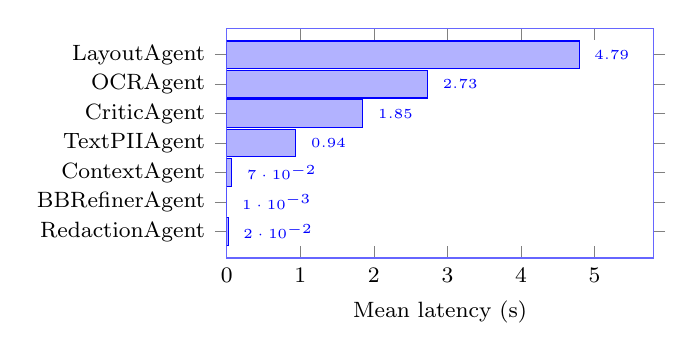
\begin{tikzpicture}
\begin{axis}[
  xbar,
  width=7cm, height=4.5cm,
  bar width=0.35cm,
  xlabel={Mean latency (s)},
  symbolic y coords={RedactionAgent,BBRefinerAgent,ContextAgent,TextPIIAgent,CriticAgent,OCRAgent,LayoutAgent},
  ytick=data,
  y tick label style={font=\footnotesize},
  x tick label style={font=\footnotesize},
  xlabel style={font=\footnotesize},
  nodes near coords,
  nodes near coords style={font=\tiny},
  every node near coord/.append style={xshift=2pt},
  xmin=0, xmax=5.8,
  enlarge y limits=0.15,
  fill=blue!30,
  draw=blue!60,
]
\addplot coordinates {
  (0.02,RedactionAgent)
  (0.001,BBRefinerAgent)
  (0.07,ContextAgent)
  (0.94,TextPIIAgent)
  (1.85,CriticAgent)
  (2.73,OCRAgent)
  (4.79,LayoutAgent)
};
\end{axis}
\end{tikzpicture}
\caption{Per-agent latency breakdown for image
  redaction (warm models). LayoutAgent (VLM
  inference) dominates at 4.79\,s (46\% of total).
  OCRAgent and CriticAgent together account for
  a further 44\%.}
\label{fig:timings}
\end{figure}

% ── Figure 4: Confusion Matrix ─────────────────
\begin{figure}[t]
\centering
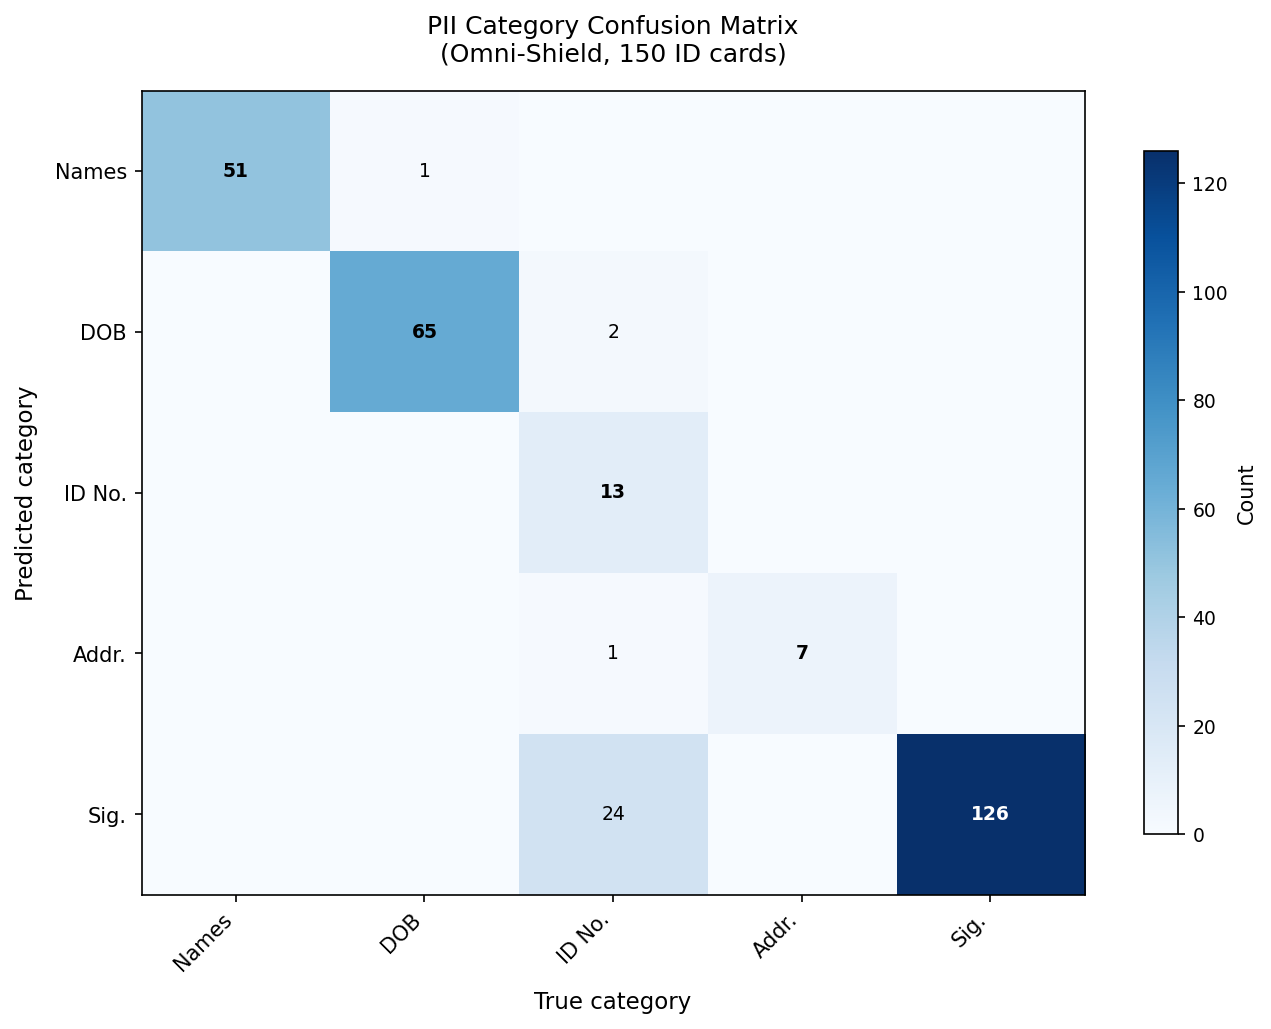
\includegraphics[width=0.85\columnwidth]
  {confusion_matrix.png}
\caption{PII category confusion matrix across
  150 test documents. False negatives (655)
  dominate over false positives (175), indicating
  that recall, not precision, is the primary
  failure mode. Date of Birth exhibits the highest
  false positive rate (61 FP against 65 TP).}
\label{fig:confusion}
\end{figure}
